\chapter{Runtime Monitoring}
As we have described in Section~\ref{sec:runtime} that there's a notable class of system, named as runtime, that are able to handle the complexity and the non compliance with the safety standard of its own AI models. These system rely their management of their complex algorithms on different solutions, one of which is known as runtime monitoring. In this scenario one of the main challenge is to obtain a certification when within the system is present a module that doesn't have a deteministic behavior, that is very complex to handle in a formal way and that can be produce some undetectable fault in the system.

One of the most practical solution to solve this problem is the \textit{runtime assurance} (RTA): we don't try to make compliance the complex module, but instead we want to predict a fault behavior of it and in this case switch to a safe module. This apporach has a high modularity: once we have obtain the certification for the whole system, we can change the AI modul without problems, because if it fails the safe fuction enter in action. Another interesting point is that that this solution cane be applies at every system level (e.g., flight controller and actuation system)~\cite{nagarajan2021astm}.

%%%%%%%%%%%%%%%%%%%%%%%%%%%%%%%%%%%%%%%%%%%%%%%%
\section{Architecture}
The idea that we described in the introduction of this Chapter, is formalized in the \textit{ASTM F3269-17} stardard (the last versione is the F3269-21, but it's to purchase). In 2017 the Advancing Standards Transforming Market (ASTM) has published a guide line to implement this behavior on unmanned airceaft system. The Figure\ref{fig:RTA_architecture} show us a schema of the architecture that was proposed.
\begin{figure}[htbp]
    \centering
    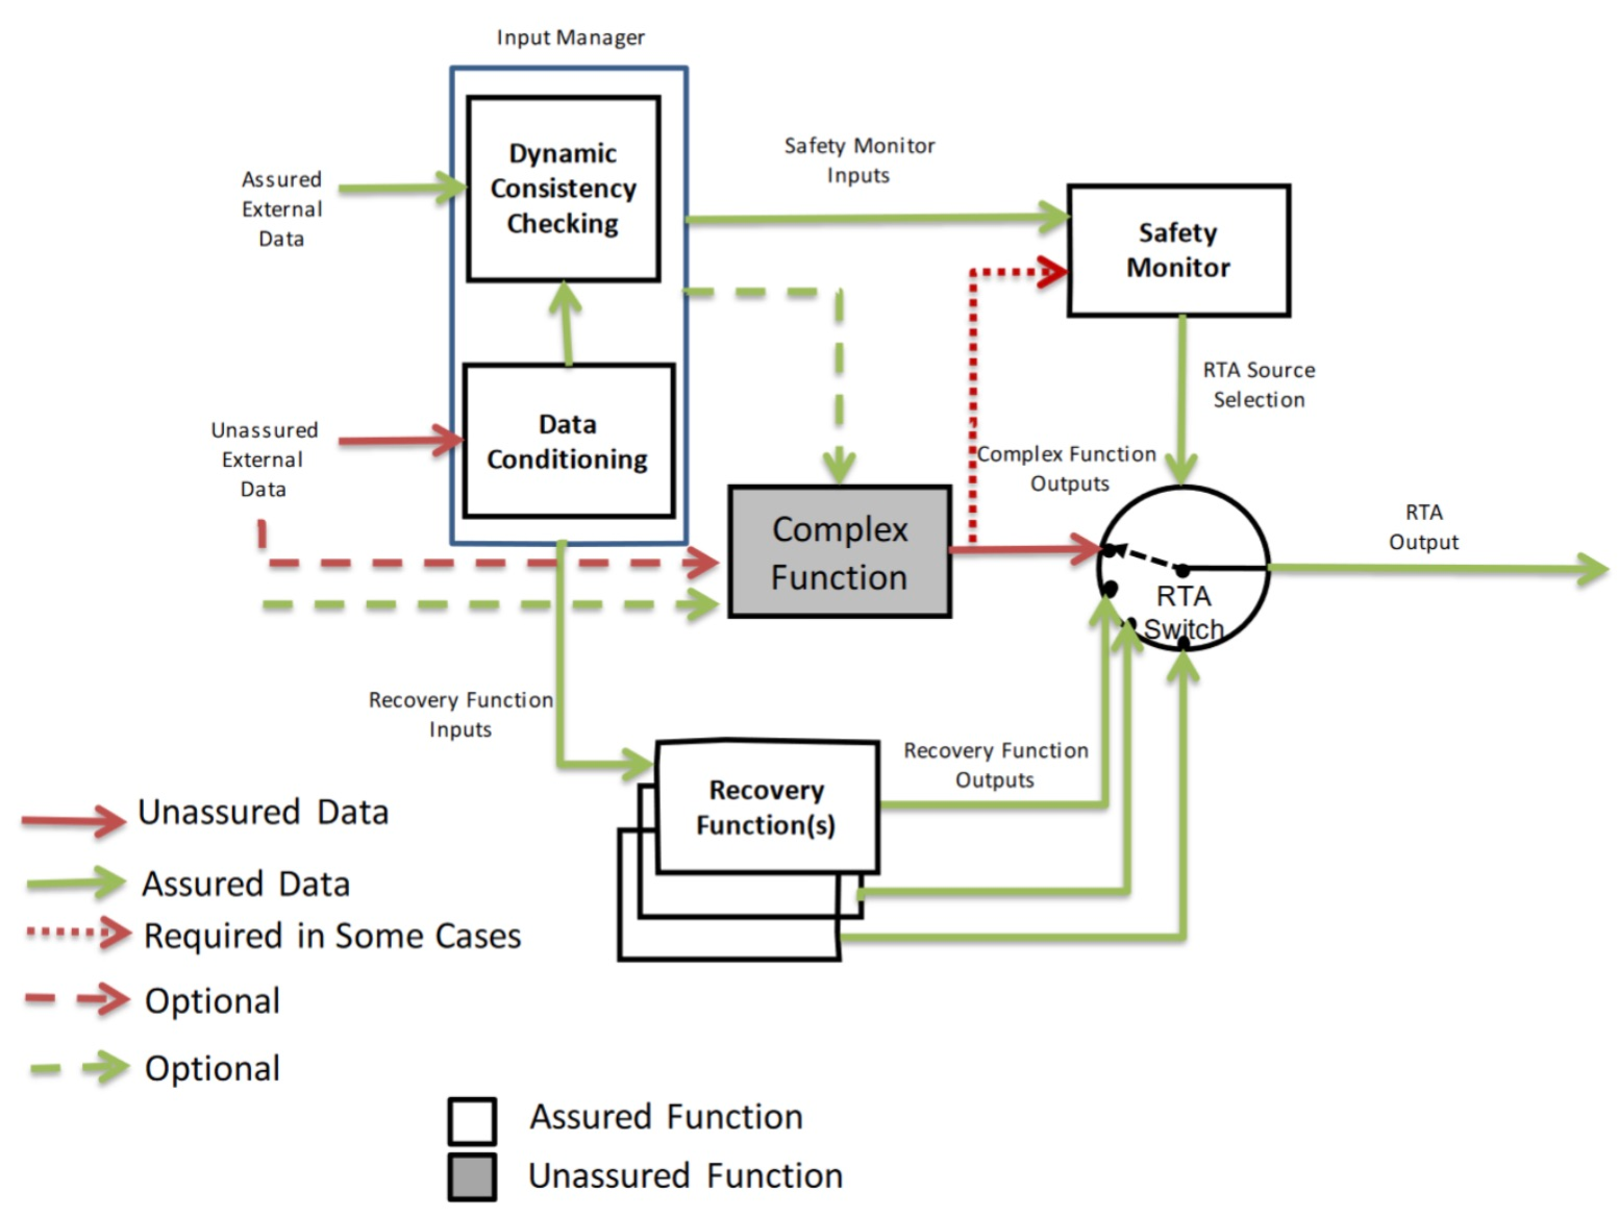
\includegraphics[max width=\textwidth, max height=0.85\textheight, keepaspectratio]{images/3-monitoring/RTA_architecture.pdf}
    \caption{RTA architecture Proposed in ASTM F3269-17~\cite{nagarajan2021astm}.}
    \label{fig:RTA_architecture}
\end{figure}

\myskip

Let's see some terms that are usefull to known:
\begin{itemize}
    \item \textbf{Data} \\
        Onviusually the data are the informations that will be treated by the system. These data can be both assered and unassured: in the first case we are reffering to the data that can be use directly from the system; in the second one we are referring to the data that must be validate throught the \textbf{Input Manager}.
    \item \textbf{Complex Function} \\
        Is the module that cannot be certificated (e.g., AI model or very complex fucntion).
    \item \textbf{Recovery Function} \\
    It's an assured function that generate a bounded output to mantain the system in a safe state if the Complex Function fails.
    \item \textbf{Safety Monitor} \\
        The assured function that is responsable to detect the fault behavior and send the command to the Switch. This module can observes both the RTA system and the Complex Function; this choice depend on the use case.
    \item \textbf{Switch} \\
        An assered fuction that recive the command of switching from the Safety Monitor and switch to the Recovery Function.
\end{itemize}

%%%%%%%%%%%%%%%%%%%%%%%%%%%%%%%%%%%%%%%%%%%%%%%%
\section{Coverage}
The coverage consept is foundamental to make working the RTA system. We start from the operative scope of the Complex Function, i.e. from the boundary of the "functionality" that the Complex Function implements. This scope is analyze from a point of view of all combination of Safety Monitor and Recovery Function (see Figure~\ref{fig:monitoring:coverage_gap}): for each operation point (i.e., functionality) of the scope there must be a monitor capable to detecting the Complex Function fail and a REcovery Function that maintains the system in a safe state.
\begin{figure}[htbp]
    \centering
    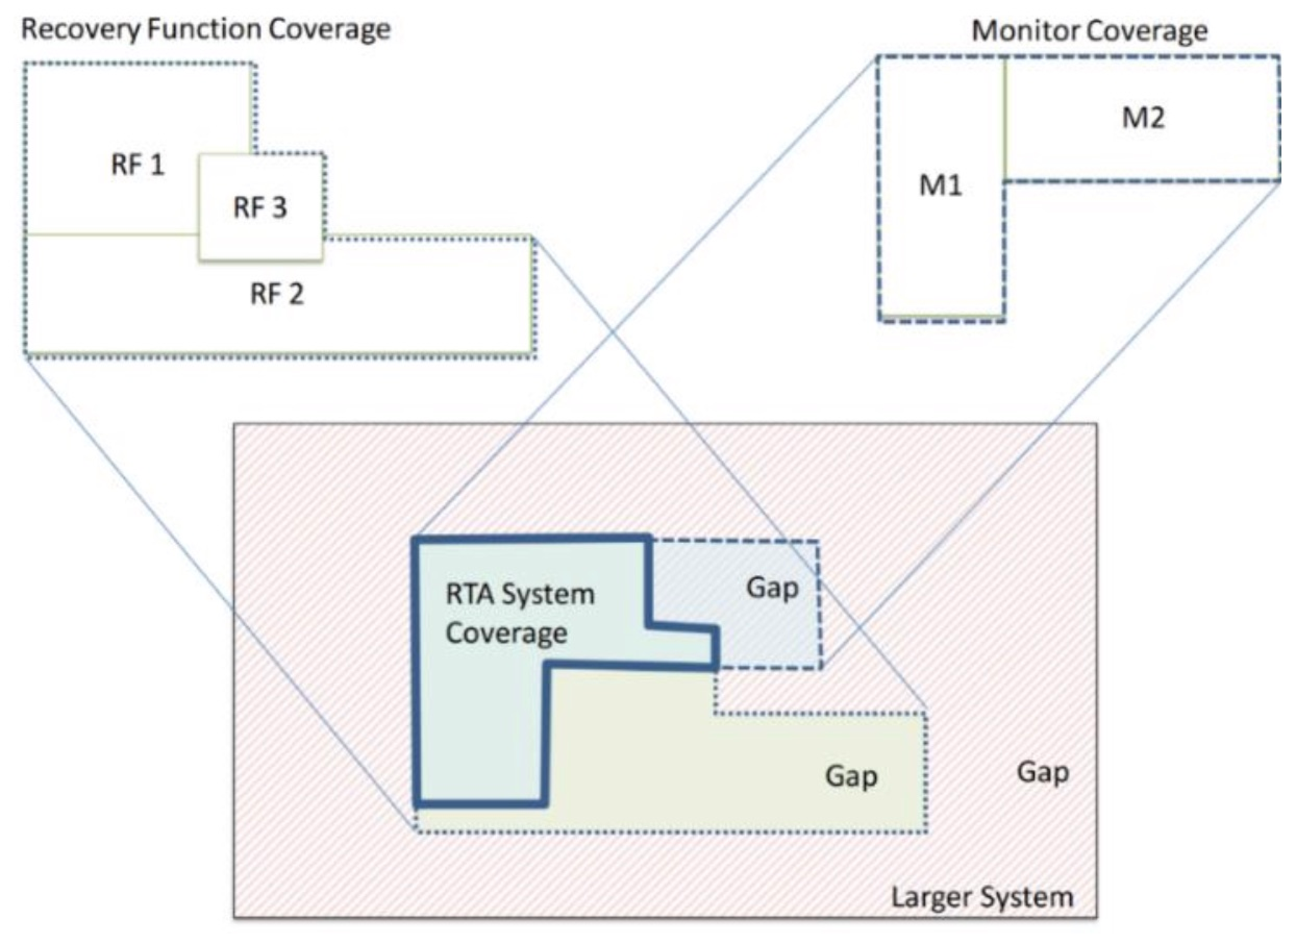
\includegraphics[max width=\textwidth, max height=0.85\textheight, keepaspectratio]{images/3-monitoring/coverage_gap.pdf}
    \caption{Gap in the Monitor and the Recovery Function~\cite{nagarajan2021astm}.}
    \label{fig:monitoring:coverage_gap}
\end{figure}

This concept of coverage brings us to have multiple Monitor where each of them have its own Recovery Function. The choice of which Monitor, and its relative Recovery Function is performed by a voter, and so we have an architecture similar to that one shown in Figure~\ref{fig:monitor:monitors_voter}.
\begin{figure}[htbp]
    \centering
    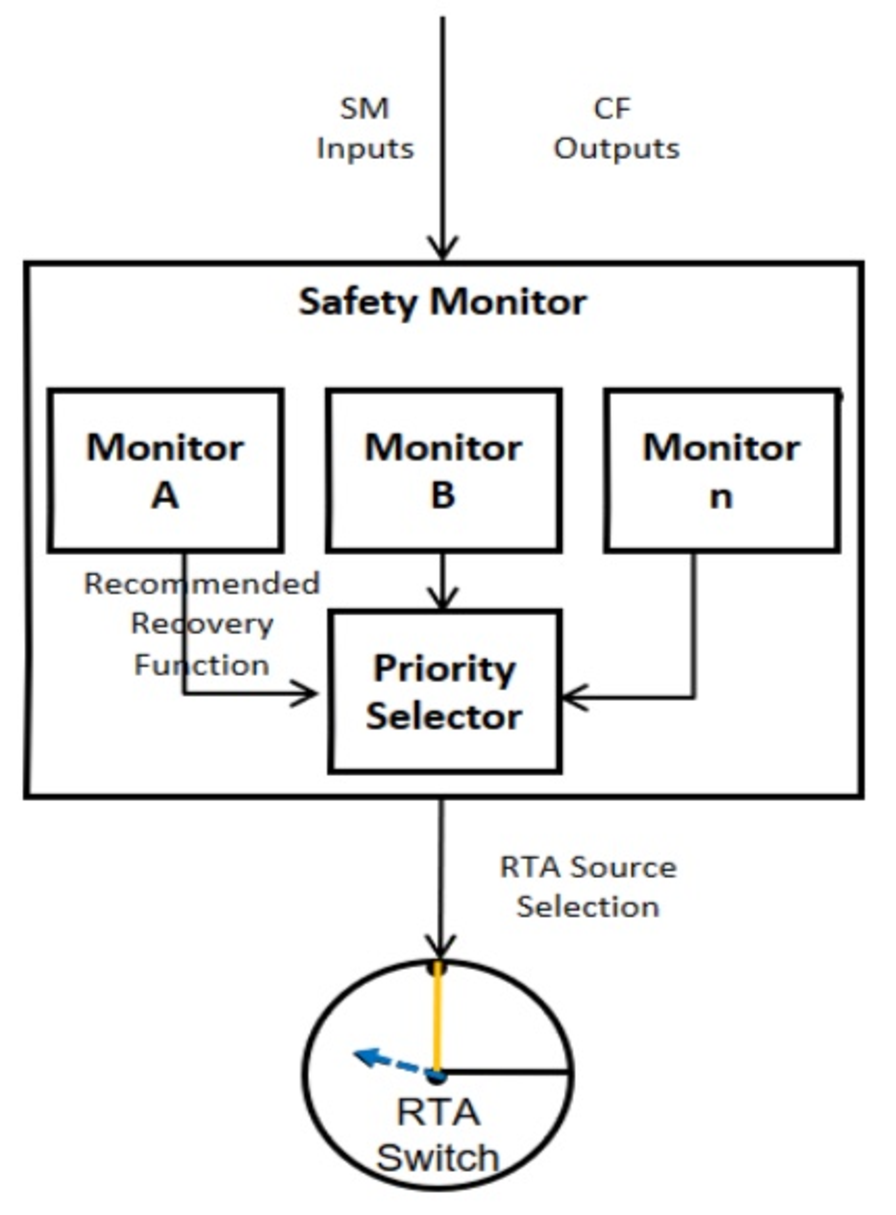
\includegraphics[max width=\textwidth, max height=.85\textheight, keepaspectratio]{images/3-monitoring/monitors_voter.pdf}
    \caption{Voter architecture with multiple Monitor~\cite{nagarajan2021astm}.}
    \label{fig:monitor:monitors_voter}
\end{figure}